\documentclass[a4paper]{article}

\usepackage[english]{babel}
\usepackage[utf8]{inputenc}
\usepackage{amsmath}
\usepackage{graphicx}
\usepackage[colorinlistoftodos]{todonotes}
\usepackage{hyperref}
\usepackage{listings}
\usepackage[numbers]{natbib}

\usepackage{booktabs} % To thicken table lines



\title{Creating Customer Segments}

\author{Uirá Caiado}

\date{\today}

\begin{document}

\maketitle

\begin{abstract}
As pointed out by \cite{Udacity}, today many companies collect vast amounts of data on their clientele and have a strong desire to understand the meaningful relationships hidden in their customer base. In this project, I will apply unsupervised learning techniques on product spending data collected for consumers of a wholesale distributor in Lisbon, Portugal. My goal is to define how best segment their customers into distinct categories. Afterwards, the segmentation found will be compared with an additional labeling. Lastly, I will suggest ways that the segmentation could assist the wholesale distributor with future service changes.
\end{abstract}

%%%%%%%%%%%%%%%%%%%%%%%%%%%%%%%%%%%%%%%%%%%%%%%%%%%%%%%%%%%%%%%%%%%%%%%%%%%%%%%%%%%%%%%%
%% INTRODUCTION
%%%%%%%%%%%%%%%%%%%%%%%%%%%%%%%%%%%%%%%%%%%%%%%%%%%%%%%%%%%%%%%%%%%%%%%%%%%%%%%%%%%%%%%%

\section{Introduction}
\label{sec:introduction}
In this section, I will give some background about the problem addressed and the goal of the project.

\subsection{Some Background}
As suggested by this article\footnote{Source: \url{http://goo.gl/aEqNpD}}, the current abundance of digital data from many sources — the web, sensors, smartphones and corporate databases — can be mined for discoveries and insights and might lead to smarter, data-driven decision-making in every field.

In this project, I will analyze a dataset containing data on various customers' annual spending amounts of diverse product categories looking for internal structure. One goal of this project is to best describe the variation in the different types of customers that a wholesale distributor interacts with. Doing so would equip the distributor with insight into how to best structure their delivery service to meet the needs of each customer.

Given that there is no previous labeling of each instance in the dataset, I will use unsupervised learning to look for such structure. As explained by \cite{Mitchell}, in this case, there is a set of $N$ observations $(x_1,x_2, ..., x_N )$ of a random vector $X$ that has a joint density $Pr(X)$. The goal is to directly infer the properties of this probability density without the help of a supervisor or teacher providing correct answers or degree-of-error for each observation.

\subsection{Getting Started}
The dataset for this project can be found on the UCI Machine Learning Repository\footnote{Source: \url{https://archive.ics.uci.edu/ml/datasets/Wholesale+customers}}. For the purposes of this project, the features \textit{'Channel'} and \textit{'Region'} will be excluded in the analysis — with focus instead on the six product categories recorded for customers. So, let's start loading the dataset:

% code snipet
\begin{lstlisting}
Wholesale customers dataset has 440 samples with 6 features
each.
\end{lstlisting}

%%%%%%%%%%%%%%%%%%%%%%%%%%%%%%%%%%%%%%%%%%%%%%%%%%%%%%%%%%%%%%%%%%%%%%%%%%%%%%%%%%%%%%%%
%% DATA EXPLORATION
%%%%%%%%%%%%%%%%%%%%%%%%%%%%%%%%%%%%%%%%%%%%%%%%%%%%%%%%%%%%%%%%%%%%%%%%%%%%%%%%%%%%%%%%


\section{Data Exploration}
\label{sec:data_exploration}
In this section, I will begin exploring the data to understand how each feature is related to each others.

\subsection{Basic Statistics}
The six labels explored are continuous and are related to the annual spending on diverse product categories. They are all expressed in in monetary units. The features are:
\begin{itemize}
\item FRESH: fresh products
\item MILK: milk products
\item GROCERY: grocery products
\item FROZEN: frozen products
\item DETERGENTS\_PAPER: detergents and paper products
\item DELICATESSEN: delicatessen products
\end{itemize}

In the Table \ref{tab:basicfacts} below can be observed a statistical description of the dataset:

\begin{table}[ht!]
\centering
\begin{tabular}{l|rrrrrr}
{} &      Fresh &      Milk &   Grocery &    Frozen & Deter. Papr. & Delicatss. \\\hline
count &     440.00 &    440.00 &    440.00 &    440.00 &           440.00 &       440.00 \\
mean  &   12000.30 &   5796.27 &   7951.28 &   3071.93 &          2881.49 &      1524.87 \\
std   &   12647.33 &   7380.38 &   9503.16 &   4854.67 &          4767.85 &      2820.11 \\
min   &       3.00 &     55.00 &      3.00 &     25.00 &             3.00 &         3.00 \\
25\%   &    3127.75 &   1533.00 &   2153.00 &    742.25 &           256.75 &       408.25 \\
50\%   &    8504.00 &   3627.00 &   4755.50 &   1526.00 &           816.50 &       965.50 \\
75\%   &   16933.75 &   7190.25 &  10655.75 &   3554.25 &          3922.00 &      1820.25 \\
max   &  112151.00 &  73498.00 &  92780.00 &  60869.00 &         40827.00 &     47943.00 \\

\end{tabular}
\caption{\label{tab:basicfacts}Statistics About The Dataset.}
\end{table}

\subsection{Selecting Samples}
\label{sec:selecting_samples}
To get a better understanding of the customers and how their data will transform through the analysis, in the Table \ref{tab:sample} I selected a few sample data points and plotted a boxplot in Figure \ref{fig:boxplot} comparing them with the distribution of each feature.

\begin{table}[ht!]
\centering
\begin{tabular}{l|rrrrrr}
{ID} &    Fresh &     Milk &  Grocery &    Frozen & Detergents & Delicatessen \\\hline
1   &  7057.00 &  9810.00 &  9568.00 &   1762.00 &          3293.00 &      1776.00 \\
271 &  2083.00 &  5007.00 &  1563.00 &   1120.00 &           147.00 &      1550.00 \\
413 &  4983.00 &  4859.00 &  6633.00 &  17866.00 &           912.00 &      2435.00 \\

\end{tabular}
\caption{\label{tab:sample}A Sample Of The Original Dataset}
\end{table}

\begin{figure}[ht!]
\centering
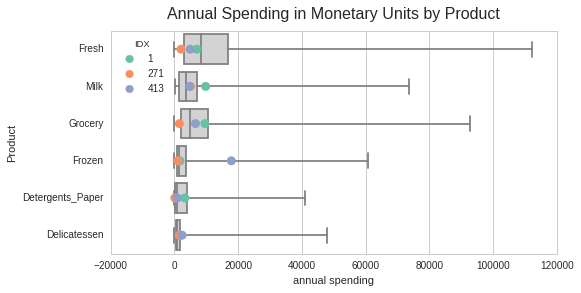
\includegraphics[width=0.85\textwidth]{figures/boxplot_features_new.png}
\caption{\label{fig:boxplot}Distribution Of The Features}
\end{figure}

Usually data expressed in money, as wealth, expenses, income and so on, are very skewed\footnote{Source: \url{https://en.wikipedia.org/wiki/Skewness}}. As can be seen above, this dataset is not different. The box shows the quartiles of the dataset while the whiskers extend to show the rest of the distribution. There are some customers who spend much more than the median, while the most of them spend around the same level (the data inside the box comprehend 50\% of the dataset).

The data point 271 spent less than 75\% of the other customers (lower quartile) in three product categories: Fresh, Groceries and detergent papers. On the another hand, it spent above the median in products relates to Milk. It could be a small coffee shop, for example. The customer $1$ could be a hotel, as it spent above or expressively above the mean in all product categories, except by Fresh. The last customer selected, 413, has spent at the fourth quartile of the distributions in two products: Frozen, that is well above the third quartile, and delicatessen. It could be a small grocery store.

\newpage
\subsection{Feature Relevance}
One interesting thought to consider is if one (or more) of the six product categories is actually relevant for understanding customer purchasing. That is to say, is it possible to determine whether customers purchasing some amount of one group of goods will necessarily buy some proportional amount of another category of products? We can make this determination by training a supervised regression learner on a subset of the data with one feature removed and then score how well that model can predict the removed feature.

The table  \ref{tab:r2} shows the $R^{2}$ when attempting to predict different features. The regressions were performed using a Decision Tree\footnote{Source: \url{http://goo.gl/JuLuJH}}. I divided the data between a test and a training set, and then took out one of the features at each iteration to be predicted by all others. Finally, I measured how well those features were relevant to replicate the hold-out column using the coefficient of determination, the $R^{2}$. This coefficient is scored between 0 and 1, with 1 being a perfect fit. A negative $R^2$ implies the model fails to fit the data.

\begin{table}[ht!]
\centering
\begin{tabular}{l|r}
{Predicted} &  Score \\\hline
Fresh            &  -0.77 \\
Milk             &   0.05 \\
Grocery          &   0.74 \\
Frozen           &  -1.41 \\
Detergents\_Paper &   0.56 \\
Delicatessen     &   0.16 \\

\end{tabular}
\caption{\label{tab:r2}The $R^{2}$ when predicting each feature}
\end{table}

As can be seen in the table above, two features, \textit{Grocery} and \textit{Detergents\_Paper}, presented a high $R^2$ score. Around $75$\% and $55$\% of the sample variation in each of the columns used as labels were explained by the other features, respectively. Looking at just this score, I would say that at least the `Grocery` might be unnecessary for identifying customers' spending habits. A good deal of the information on the variability of this feature is contained in others. On the other hand, \textit{Fresh} and \textit{Frozen} presented negative $R^2$, what indicates that the information from them could not be retrieved using other features. In spite of those finds, it is important to point out that low R-squared values\footnote{Source: \url{http://goo.gl/rRAVdJ}} are not inherently bad. This score should always be analyzed in conjunction with other measurements. So, in the next session, I will inspect those relationships visually.


\subsection{Visualize Feature Distributions}

To get a better understanding of the dataset, in the figure \ref{fig:scatter_matrix} I am going to plot a scatter matrix of each of the six product features present in the data.

\newpage
\begin{figure}[ht!]
\centering
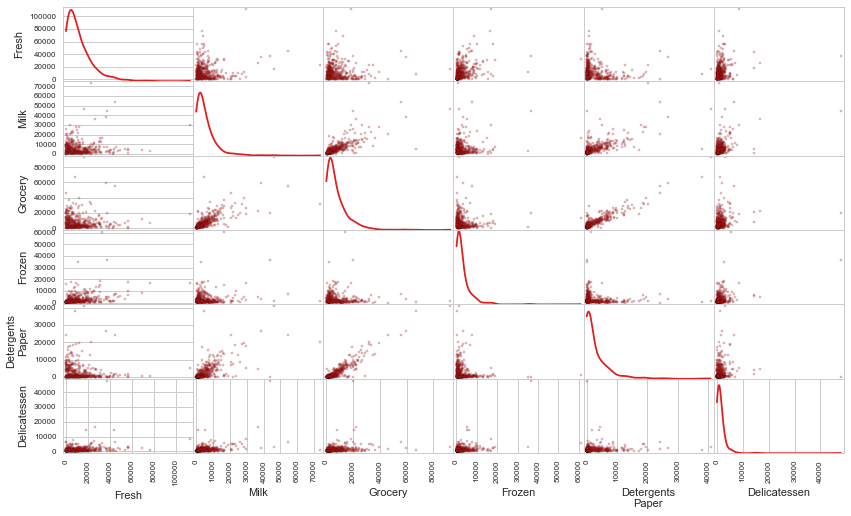
\includegraphics[width=0.75\textwidth]{figures/scatter_matrix.png}
\caption{\label{fig:scatter_matrix}How the Features Correlated}
\end{figure}

In the main diagonal\footnote{Source: \url{http://www.mathwords.com/m/main_diagonal.htm}} is plotted the distribution of each one. As suggested in section \ref{sec:selecting_samples}, the features are very skewed, apparently showing a Log Normal Distribution\footnote{Source: \url{http://mathworld.wolfram.com/LogNormalDistribution.html}}. As the most of the data points are lying in the bottom corner of the charts, it is a little cumbersome to judge the relationships. Below, I am going to look at the correlation matrix of the features using a heat map.

\begin{figure}[ht!]
\centering
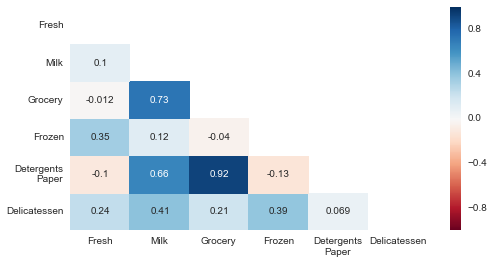
\includegraphics[width=0.75\textwidth]{figures/heatmap.png}
\caption{\label{fig:heatmap}Heat Map Of The Correlation Matrix}
\end{figure}

The scatter plot between \textit{Grocery} and \textit{Detergents\_Paper} presented a curious linear relationship. It might suggest that they are complements\footnote{Source: \url{http://www.investopedia.com/terms/c/complement.asp}} to each other. That is, they are consumed in conjunction with other, or they can be complements to a third variable. For example, the \textit{Milk} category seems to be slightly correlated with those features. The strength of this relationship can be confirmed by the correlation between the two features ($0.92$).

The \textit{Fresh} and \textit{Frozen} categories are slightly ($0.35$) correlated with each other, as the pairs \textit{Delicatessen} and  \textit{Frozen} ($0.39$) and \textit{Delicatessen} and \textit{Milk} ($0.41$). In the next section, I will deal with the apparently log distribution of the dataset.

%%%%%%%%%%%%%%%%%%%%%%%%%%%%%%%%%%%%%%%%%%%%%%%%%%%%%%%%%%%%%%%%%%%%%%%%%%%%%%%%%%%%%%%%
%% DATA PREPROCESSING
%%%%%%%%%%%%%%%%%%%%%%%%%%%%%%%%%%%%%%%%%%%%%%%%%%%%%%%%%%%%%%%%%%%%%%%%%%%%%%%%%%%%%%%%

\section{Data Preprocessing}
\label{sec:data_preprocessing}
In this section, I will preprocess the data to create a better representation of customers by performing a scaling on the data and detecting (and possibly removing) outliers. Preprocessing data is often times a critical step in assuring that results you obtain from your analysis are significant and meaningful.


\subsection{Feature Scaling}
If data is not normally distributed, especially if the mean and median vary significantly (indicating a large skew), it is most often appropriate\footnote{Source: \url{http://econbrowser.com/archives/2014/02/use-of-logarithms-in-economics}} to apply a non-linear scaling — particularly for financial data. One way to achieve this scaling is by using a Box-Cox test\footnote{Source: \url{http://scipy.github.io/devdocs/generated/scipy.stats.boxcox.html}}, which calculates the best power transformation of the data that reduces skewness. A simpler approach which can work in most cases would be applying the natural logarithm, that I will use below

\begin{figure}[ht!]
\centering
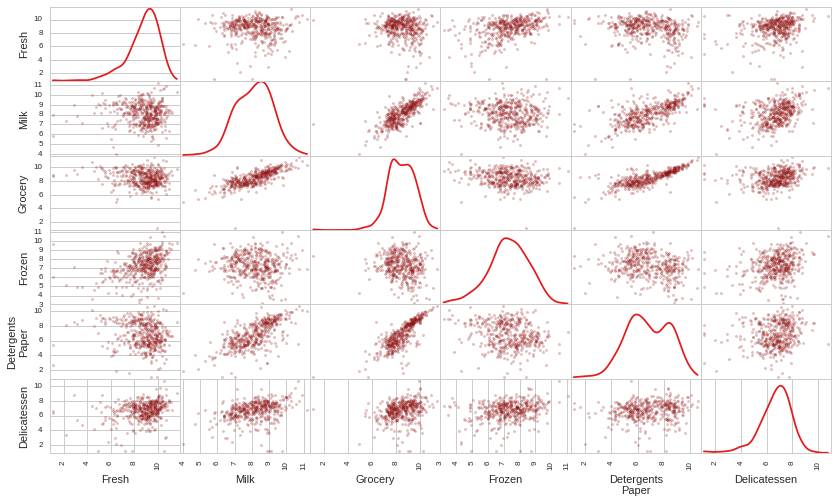
\includegraphics[width=0.75\textwidth]{figures/scatter_matrix_log.png}
\caption{\label{fig:log_scatter_matrix}How the Log-Transformed Features Correlated}
\end{figure}

After applying a natural logarithm scaling to the data, the distribution of each feature appears much more normal. Now it is clear that there is a stronger relationship between the pairs of features \textit{Grocery} and \textit{Milk} and \textit{Grocery} and `Detergents and Paper`. \textit{Milk} and \textit{Detergents and Paper} are somewhat weaker but still presented a substantial correlation.

Below can be seem how the sample data has changed after having the natural logarithm applied to it.

\begin{table}[ht!]
\centering
\begin{tabular}{l|rrrrrr}
{ID} &    Fresh &     Milk &  Grocery &    Frozen & Detergents & Delicatessen \\\hline
1   &  8.861775 &  9.191158 &  9.166179 &  7.474205 &          8.099554 &      7.482119 \\
271 &  7.641564 &  8.518592 &  7.354362 &  7.021084 &          4.990433 &      7.346010 \\
413 &  8.513787 &  8.488588 &  8.799812 &  9.790655 &          6.815640 &      7.797702 \\

\end{tabular}
\caption{\label{tab:log_sample}A Sample Of The Original Dataset}
\end{table}

Looking at the numbers transformed like that, without any reference, is a little difficult to interpret. In the next subsection, I will visualize the data in a boxplot.


\subsection{Outlier Detection}

Detecting outliers in the data is extremely important in the data preprocessing step of any analysis. The presence of outliers can often skew results which take into consideration these data points. There are many "rules of thumb" for what constitutes an outlier in a dataset. Here, I will use Tukey's Method for identfying outliers\footnote{Source: \url{http://goo.gl/FWfWnp}}: An *outlier step* is calculated as 1.5 times the interquartile range (IQR). A data point with a feature that is beyond an outlier step outside of the IQR for that feature is considered abnormal. The following summary shows the number of outliers by feature and the data points that were considered abnormal for more than one feature.

% code snipet
\begin{lstlisting}
Number of Data points considered outliers for the feature

Fresh             	16                
Milk              	4                 
Grocery           	2                 
Frozen            	10                
Detergents_Paper  	2                 
Delicatessen      	14                
-------------------------
TOTAL: Outliers: 48 | Unique Outliers: 42


Data points considered outliers for more than one feature:
\end{lstlisting}

\begin{table}[ht!]
\centering
\begin{tabular}{l|rrrrrrr}
{ID} &    Fresh &     Milk &  Grocery &    Frozen & Detergents & Delicatessen & count \\\hline
128 &  4.9416 &  9.0878 &   8.2488 &  4.9558 &          6.9679 &      1.0986 &      2 \\
154 &  6.4329 &  4.0073 &   4.9199 &  4.3174 &          1.9459 &      2.0794 &      3 \\
65  &  4.4426 &  9.9503 &  10.7326 &  3.5835 &         10.0953 &      7.2605 &      2 \\
66  &  2.1972 &  7.3356 &   8.9115 &  5.1647 &          8.1513 &      3.2958 &      2 \\
75  &  9.9232 &  7.0361 &   1.0986 &  8.3909 &          1.0986 &      6.8824 &      2 \\

\end{tabular}
\caption{\label{tab:outliers}A Sample Of The Log-Transformed Dataset}
\end{table}

There are 48 outliers in the dataset and 42 are unique. 5 data points were considered outliers for more than one feature. One of the them was abnormal to three features, as can be seen in the \textit{count} column in the table \ref{tab:outliers}. To decide which data point should be removed, I am going to plot a boxplot showing where these 5 data points are located considering the dataset without all the 42 outliers.

\begin{figure}[ht!]
\centering
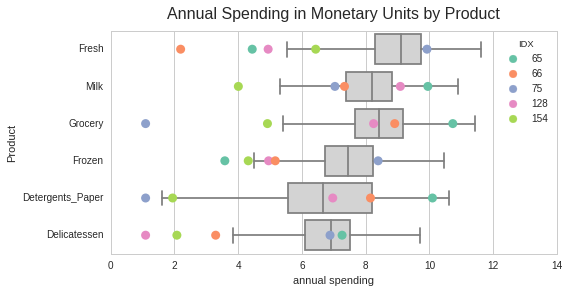
\includegraphics[width=0.75\textwidth]{figures/boxplot_features_log.png}
\caption{\label{fig:log_boxplot}Distribution Of The Log-Transformed Features}
\end{figure}

I am going to exclude the client IDs 75, 66, 128 and 154 from the dataset. As can be seen in the figure \ref{fig:log_boxplot}, the 75 is far away from the lower whiskers of the \textit{Grocery} category distribution. It is the same to the ID 128 data point in the \textit{Delicatessen} category and to the ID 66 in \textit{Fresh}. Lastly, I will exclude the 154 because was considered outlier for 3 groups. Despite that the ID 66 was found to be abnormal for two categories, I will not exclude it because it was not so far away from the lower whisker of the categories that it was considered an outlier.

%%%%%%%%%%%%%%%%%%%%%%%%%%%%%%%%%%%%%%%%%%%%%%%%%%%%%%%%%%%%%%%%%%%%%%%%%%%%%%%%%%%%%%%%
%% FEATURE TRANSFORMATION
%%%%%%%%%%%%%%%%%%%%%%%%%%%%%%%%%%%%%%%%%%%%%%%%%%%%%%%%%%%%%%%%%%%%%%%%%%%%%%%%%%%%%%%%

\section{Feature Transformation}
\label{sec:feature_transformation}
In this section I will use principal component analysis (PCA) to draw conclusions about the underlying structure of the wholesale customer data. Since using PCA on a dataset calculates the dimensions which best maximize variance, we will find which compound combinations of features best describe customers.

\subsection{PCA}

Now that the data has been scaled to a more normal distribution and has had any necessary outliers removed, I will apply PCA to the new dataset to discover which dimensions about the data best maximize the variance of features involved. In addition to finding these dimensions, PCA will also report the \textit{explained variance ratio} of each dimension — how much variance within the data is explained by that dimension alone. Note that a component (dimension) from PCA can be considered a new "feature" of the space, however it is a composition of the original features present in the data.

\begin{figure}[ht!]
\centering
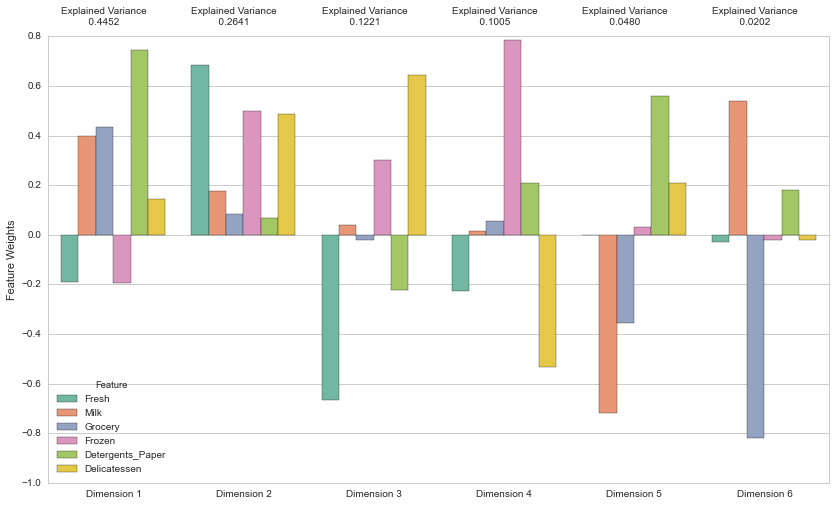
\includegraphics[width=0.75\textwidth]{figures/pca_results.png}
\caption{\label{fig:pca_results}PCA Results}
\end{figure}

As shown in the Figure above, together the 6 components explain 100\% of variance in the dataset. Combining\footnote{Source: \url{https://goo.gl/cz10xK}} all PCs would form a coordinate system where we could graph each point from the original data. More than 70\% of the variance was explained by the first two principal components. The first four explained more than 93\% of the variance.

The principal components of a dataset can be understood as new compound features, where each PC is a weighted linear combination of the original features. In the first component, for instance, \textit{Detergent\_Paper} had a strong positive effect on the PC value, followed by \textit{Grocery} and \textit{Milk}. \textit{Delicatessen} also increased the PC value, but isn't very expressive. \textit{Fresh} and \textit{Frozen} slightly decreased the PC value. Curiously, in the second component, the primary features were \textit{Fresh}, \textit{Frozen} and \textit{Delicatessen}. The other features slightly increased the PC value.

It means that if a customer buys more \textit{Detergent\_Paper} items, it follows that there is a larger increase in the feature \textit{Dimension 1} and a smaller increase in the \textit{Dimension 2}. Also, if this same customer buys more \textit{Fresh} items, it would just cause a lower decrease in the \textit{PC1},but would result in a larger increase in \textit{PC2}. As the first two PCs represent almost 70\% of the variance, we would have a decent grasp where this customer lies in the original feature space looking just at this two features.

In the third dimension of this new feature space (the principal components), \textit{Fresh} presented an enormous negative effect on the PC value, while \textit{Delicatessen} strongly increased the value. \textit{Frozen} strongly increased the fourth dimension, while \textit{Delicatessen} had the opposite effect.

The table \ref{tab:sample_transformed_1} shows how the log-transformed sample data has changed after having a PCA transformation applied to it in six dimensions.

\begin{table}[ht!]
\centering
\begin{tabular}{l|rrrrrr}
{ID} &  Dim. 1 &  Dim. 2 &  Dim. 3 &  Dim. 4 &  Dim. 5 &  Dim. 6 \\\hline
1   &       1.7537 &       0.8680 &       0.2256 &       0.0077 &      -0.1177 &       0.2111 \\
271 &      -1.3268 &      -0.7392 &       1.5119 &      -0.7648 &      -0.7701 &       0.8154 \\
413 &       0.0157 &       1.6981 &       1.6267 &       1.4426 &      -0.0606 &      -0.1465 \\

\end{tabular}
\caption{\label{tab:sample_transformed_1}Log-Transformed sample Using 6 Dimensions Transformation}
\end{table}

\subsection{Dimensionality Reduction}

When using principal component analysis, one of the main goals is to reduce the dimensionality of the data — in effect, reducing the complexity of the problem. Dimensionality reduction comes at a cost: Fewer dimensions used implies less of the total variance in the data is being explained. Because of this, the \textit{cumulative explained variance ratio} is extremely important for knowing how many dimensions are necessary for the problem. Additionally, if a significant amount of variance is explained by only two or three dimensions, the reduced data can be visualized afterwards.

The table \ref{tab:sample_transformed_2} shows how the log-transformed sample data has changed after having a PCA transformation applied to it using only two dimensions. Observe how the values for the first two dimensions remains unchanged when compared to a PCA transformation in six dimensions.

\begin{table}[ht!]
\centering
\begin{tabular}{l|rr}
{ID} &  Dimension 1 &  Dimension 2 \\\hline
1 &       1.7537 &       0.8680 \\
271 &      -1.3268 &      -0.7392 \\
413 &       0.0157 &       1.6981 \\

\end{tabular}
\caption{\label{tab:sample_transformed_2}Log-Transformed sample Using 2 Dimensions Transformation}
\end{table}

% bla 

% \begin{figure}[ht!]
% \centering
% 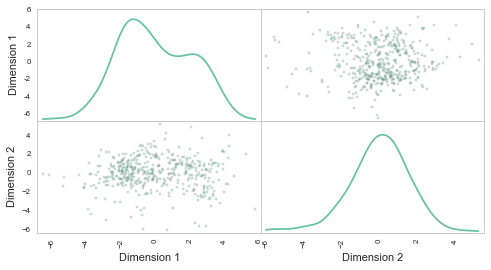
\includegraphics[width=0.75\textwidth]{figures/scatter_after_pca.png}
% \caption{\label{fig:scatter_pca}How Principal Components Are Distributed}
% \end{figure}

% bla

%%%%%%%%%%%%%%%%%%%%%%%%%%%%%%%%%%%%%%%%%%%%%%%%%%%%%%%%%%%%%%%%%%%%%%%%%%%%%%%%%%%%%%%%
%% CLUSTERING
%%%%%%%%%%%%%%%%%%%%%%%%%%%%%%%%%%%%%%%%%%%%%%%%%%%%%%%%%%%%%%%%%%%%%%%%%%%%%%%%%%%%%%%%

\section{Clustering}
\label{sec:clustering}
In this section, I will introduce the EM algorithm and use it to explain the difference between the K-Means and Gaussian Mixture Model (GMM) clustering algorithm. I will use them to identify the various customer segments hidden in the data. Then, I will choose one to recover specific data points from the clusters to understand their significance by transforming them back into their original dimension and scale. 

\subsection{Comparing GMM To K-Means Algorithm}

The GMM uses the Estimation-Maximization (EM) algorithm for fitting mixture-of-Gaussian models, using a Gaussian distribution in the Estimation step with covariance matrix between the different clusters. The KMeans\footnote{Source: \url{http://goo.gl/7dsCl3}} is equivalent to the EM algorithm when the covariance matrix between the clusters is small, all equal and diagonal.

That said, I am going to explain the Estimation-Maximization algorithm to show where the main difference between GMM and K-mean algorithm comes from. The EM\footnote{Source: \url{http://goo.gl/qwyaYM}} algorithm (\cite{Mitchell}) is a widely used approach to learning in the presence of unobserved variables.

So, let $X = \{x_1, ..., x_m\}$ denote a set of observed data in a set of $m$ independently drawn instances and $Z = \{z_1, ..., z_m\}$ unobserved data (latent variables) in these same instances. Let $Y = X \cup Z$ be a random variable\footnote{Source: \url{https://www.mathsisfun.com/data/random-variables.html}} representing the full data. $h$ is the hypothesized values to the parameters $\theta$, that governs the probability distribution from $Y$. In GMM algorithm, it represents the $\mu$ and $\sigma$ of the Gaussian Distribution. ${h}'$ is the revised parameters.

The EM algorithm searches for the maximum likelihood hypothesis ${h}'$ by seeking the parameters that maximize $E[\ln \, P(Y |{h}')]$. As it is an expectation, it is averaging over the possible values of the latent variables $Z$, weighting each $z$ according to its probability. Thus, the following steps are repeated until convergence:

\textbf{step 1} Estimation(E) step: Calculate $Q({h}'|h)$ using current hypothesis $h$ and the observed data $X$ to estimate the probability distribution over $Y$.

$$Q({h}'|h) \leftarrow E[\ln P(Y | {h}')| h, \, X] $$

\textbf{step 2} Maximization(M) step: Replace hypothesis $h$ by the hypothesis ${h}'$ that maximizes this $Q$ function.

$$h \leftarrow \underset{{h}'}{\arg \max} \, Q({h}'|h)$$

Where $\ln P(Y | {h}') = ln \prod p(y_i| {h}') = \sum ln\, p(y_i| {h}')$. As stated before, the hypothesis ${h}'$ represents the values to the parameters $\theta$ of the distribution of each cluster in the data set (we need to provide the number of clusters beforehand). So, we are summing up the log-probability of each particular instance be part of one of these clusters. As the clusters in GMM might covariate in a meaningful way and in K-means not, the main difference between both is that an instance can be "shared" by more than one group at a time in GMM (due to the covariance matrix). It uses a probabilistic approach to classify the data. On the other hand, the K-means performs a kind of "hard" assignment, attributing each instance to a particular cluster.

One advantage of the K-means over GMM is the simplicity -  It basically minimizes the sum of Euclidean distances between each point, while the other needs to estimate the $\mu$, $\sigma$ of each cluster. It leads the K-means to be a relatively faster algorithm and probably will work better when the data is clearly separable. In the next subsection, I will test both algorithms to choose between them.

\subsection{Creating Clusters}

Depending on the problem, the number of clusters that you expect to be in the data may already be known. When the number of clusters is not known \textit{a priori}, there is no guarantee that a given number of clusters best segments the data, since it is unclear what structure exists in the data — if any. However, we can quantify the "goodness" of a clustering by calculating each data point's \textit{silhouette coefficient}. This coefficient\footnote{Source: \url{http://http://goo.gl/m7XIrQ}} measures how similar a data point is to its assigned cluster, from -1 (dissimilar) to 1 (similar). In the figure \ref{fig:silhouette}, I am going to calculate the mean silhouette coefficient to K-Means and GMM using different number of clusters. Also, I will test different covariance structures to GMM.

\begin{figure}[ht!]
\centering
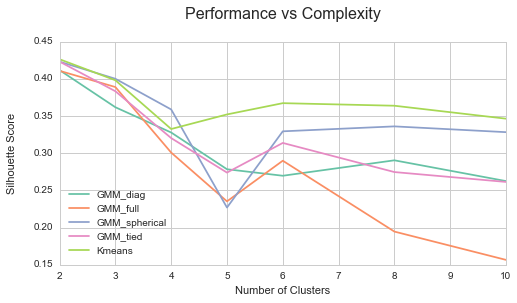
\includegraphics[width=0.75\textwidth]{figures/silhouette_score.png}
\caption{\label{fig:silhouette}Silhouette Coefficient}
\end{figure}

\begin{table}[ht!]
\centering
\begin{tabular}{l|rrrrr}
{\# } &  GMM\_diag &  GMM\_full &  GMM\_spherical &  GMM\_tied &    K-means \\\hline
2        &  0.411629 &  0.410722 &       0.422988 &  0.423095 &  0.426297 \\
3        &  0.361776 &  0.388915 &       0.400039 &  0.383261 &  0.398013 \\
4        &  0.327802 &  0.300845 &       0.358788 &  0.320299 &  0.332522 \\
5        &  0.278441 &  0.235268 &       0.226959 &  0.273933 &  0.352106 \\
6        &  0.269692 &  0.289899 &       0.329408 &  0.313793 &  0.367256 \\
8        &  0.290437 &  0.194652 &       0.336048 &  0.274649 &  0.363809 \\
10       &  0.262524 &  0.156622 &       0.328277 &  0.261379 &  0.346406 \\

\end{tabular}
\caption{\label{tab:centroids}Silhouette Coefficient By Number Of Centroids}
\end{table}

As can be seen in Table \ref{tab:centroids}, the best K-means silhouette coefficient (around $0.4263$) occurred when it was set with two clusters. This setting outperformed all the GMM methods configurations tested. I am going to use this clustering algorithm in the Figure \ref{fig:clustering_1} to split the dataset into two groups. I will also plot the sample and the centroids, denoted numbers.

\begin{figure}[ht!]
\centering
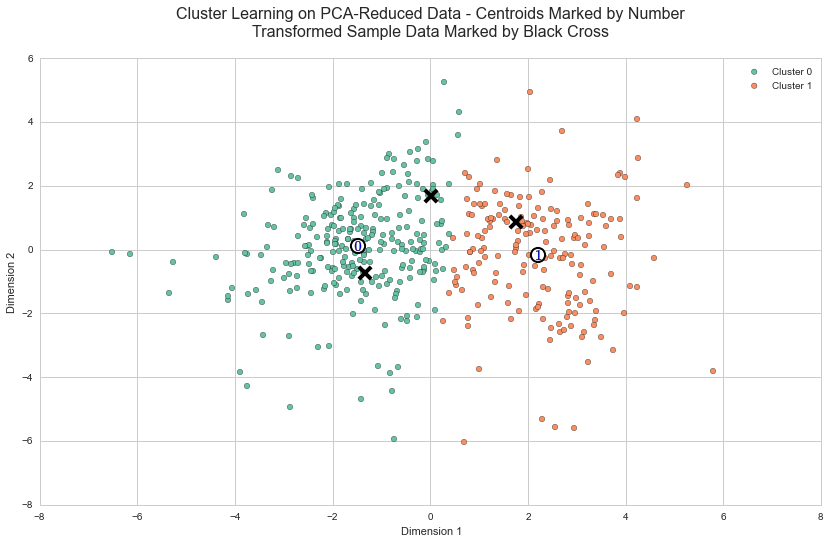
\includegraphics[width=0.75\textwidth]{figures/clustering_1.png}
\caption{\label{fig:clustering_1}Clusters Visualization}
\end{figure}

\subsection{Data Recovery}

Each cluster present in the visualization in the Figure \ref{fig:clustering_1} has a central point. These centers (or means) are not specifically data points from the data, but rather the \textit{averages} of all the data points predicted in the respective clusters. For the problem of creating customer segments, a cluster's center point corresponds to the average customer of that segment. Since the data is currently reduced in dimension and scaled by a logarithm, we can recover the representative customer spending from these data points by applying the inverse transformations.


\begin{table}[ht!]
\centering
\begin{tabular}{l|rrrrrr}
{Segment} &  Fresh &  Milk &  Grocery &  Frozen &  Deterg. Paper &  Delicatessen \\\hline
0 &   9041 &  1924 &     2508 &    2116 &               301 &           689 \\
1 &   3754 &  7970 &    12296 &     904 &              4666 &          1027 \\

\end{tabular}
\caption{\label{tab:centrois_Recov}Representative Mean Customer Spending}
\end{table}

The \textit{average customer} of Segment $0$ has consumed more than $50\%$ of the data set on Fresh, Grocery, and Frozen Categories. On the other hand, he has consumed less than $50\%$ in the other categories. On Detergents and Paper, he has spent around $25\%$. This cluster could includes costumers like restaurants, for instance. The \textit{average customer} of Segment $1$ has consumed well above $75\%$ on Milk and Grocery and has spent around $25\%$ of the dataset on Frozen category. It could include costumers like coffee shops and grocery stores.

Looking at the predictions for each sample point, the segmentation performed is consistent with what I have thought. 

When I analyzed the Figure \ref{fig:boxplot}, I have mentioned that the sample points $1$ spent well above the median in \textit{Milk}, \textit{Grocery} and \textit{Detergents\_Paper} categories. It would make this sample point match the Cluster $1$ center. The sample point $271$ match Cluster $0$, as it spent well below the median in \textit{Detergents\_Paper} category, the primary driver of this Segment. Finally, the $413$ also match the Cluster $0$, as it is high \textit{Frozen} and low in \textit{Fresh}, that is the opposite of the mains drivers of the Segment $1$. So, these data points should be assign to the clusters $\{ 1, 0, 0\}$, as the algorithm has assigned.

%%%%%%%%%%%%%%%%%%%%%%%%%%%%%%%%%%%%%%%%%%%%%%%%%%%%%%%%%%%%%%%%%%%%%%%%%%%%%%%%%%%%%%%%
%% CONCLUSION
%%%%%%%%%%%%%%%%%%%%%%%%%%%%%%%%%%%%%%%%%%%%%%%%%%%%%%%%%%%%%%%%%%%%%%%%%%%%%%%%%%%%%%%%

\section{Conclusion}
\label{sec:conclusion}

As stated in Section \ref{sec:introduction}, the goal here is to describe the variation in the different types of customers. The companies often run A/B tests\footnote{Source: \url{https://en.wikipedia.org/wiki/A/B_testing}} when making small changes to their products or services, where two versions (A and B) are compared, which are identical except for one variation that might affect a user's behavior.

The analysis suggested that there are two customers groups in the dataset. So, if the wholesale distributor wanted to change its delivery service from 5 days a week to 3 days a week, he could take two samples from each group and run an A/B test to see how each segment would respond to the change in the delivery time. The Segment 0 that spends heavily in Fresh and Grocery might react differently to the delivery strategy than the Segment 1, for example. Thus, the segmentation would help the wholesale distributor choosing between delivery strategies based on the purchases behavior of a particular customer.

The clusters found also could be used as new features in the dataset. As some features may be affected by the customer segment, the groups could be used as dummy variables in a supervised learning task, for example. So, if the wholesale distributor wanted to predict the sales in another product category, the segmentation found would be used as one of the features to train the model and could improve the performance of the algorithm.

Finally, at the beginning of this project, it was discussed that the \textit{Channel} and \textit{Region} features would be excluded from the dataset so that the customer product categories were emphasized in the analysis. In the Figure \ref{fig:clustering_2}, I am going to reintroduce the \textit{Channel} feature to the dataset. An interesting structure emerges when considering the same PCA dimensionality reduction applied earlier on to the original dataset.

\begin{figure}[ht!]
\centering
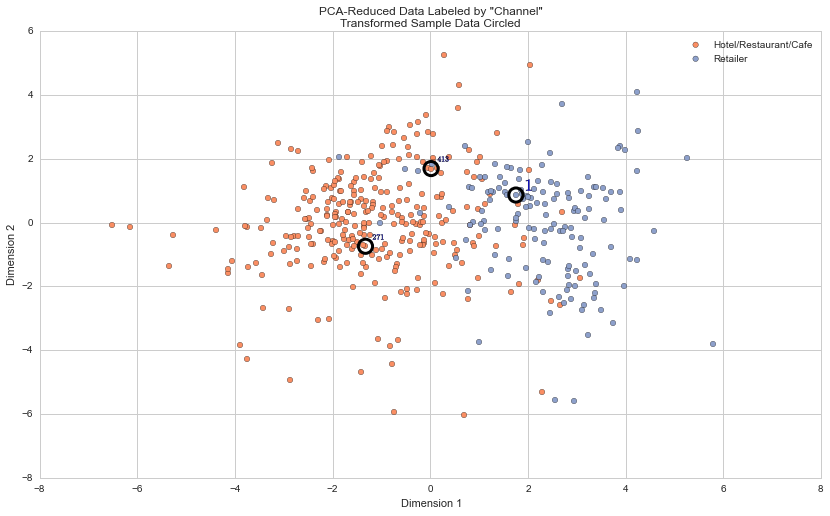
\includegraphics[width=0.75\textwidth]{figures/clustering_2.png}
\caption{\label{fig:clustering_2}Cluster Visualization}
\end{figure}

The K-means successfully identified the number of the main categories in the dataset. Although the groups are not clearly separable, as expected by the algorithm, I believe that it worked fine. The underlying distribution of Hotel/Restaurant/Cafe customers to Retailer customers suggests that some of them share characteristics of each other. For instance, a big hotel could consume like a retailer and a retailer can be specialized in sell products to hotels, assuming the same behavior of the last one. So, I believe that these classifications are consistent enough with the previous finds.

%%%%%%%%%%%%%%%%%%%%%%%%%%%%%%%%%%%%%%%%%%%%%%%%%%%%%%%%%%%%%%%%%%%%%%%%%%%%%%%%%%%%%%%%
%% REFLECTION
%%%%%%%%%%%%%%%%%%%%%%%%%%%%%%%%%%%%%%%%%%%%%%%%%%%%%%%%%%%%%%%%%%%%%%%%%%%%%%%%%%%%%%%%

\section{Reflection}
\label{sec:reflection}
Given that the dataset is not clearly separable, would be interesting to see how a soft clustering assignment would have performed. Nevertheless, for the purpose of this project, the segmentation found would be useful to best structure the delivery service of the wholesale distributor.




\bibliographystyle{plain}
% or try abbrvnat or unsrtnat
\bibliography{bibliography/biblio.bib}
\end{document}
